\chapter{Appendices for Chapter \ref{ch:Borregaard_PRL2015}}
\label{app:Borregaard_PRL2015}

This appendix describes the details of the
perturbation theory and the derivation of the effective Hamiltonian
$\hat{H}_{\text{eff}}$ and effective Lindblad operators. We describe the
situation both with and without a two-photon drive. Furthermore, we present the
results of a numerical simulation of the full dynamics of the gates to verify
the results found with perturbation theory and address the question of how
strong a drive we can allow for. In the end, this determines the gate time as
described in the article. Finally we discuss of the additional errors described
in the final part of the article.

\section{Perturbation theory}

We will now give the details of the perturbation theory and the derivation of
the effective operators together with the success probabilitites, gate times and
gate errors (see \tabref{tab:table1}). Our perturbation theory is based on the
effective operator formalism described in Ref.~\cite{Florentin}.
 
\begin{table} [h]
\centering
\begin{tabular}{|c|c|c|c|c|}
\hline
Gate & Origin of error & Error & Probability & Time  \\ \hline CZ-gate &
\specialcell{$\gamma_{g}=0$
\\$\gamma_{g}>0$} & \specialcell{$0$\\$\sim
\frac{\gamma_{g}}{\gamma\sqrt{C}}$} & $\sim 1-\frac{6}{\sqrt{C}}$ &
$\sim\frac{15\pi\sqrt{C}\gamma}{2\Omega^{2}}$\\ \hline Toffoli &
\specialcell{$\Gamma_{i}\neq\Gamma_{j}$\\$\gamma_{g}>0$} &
\specialcell{$\lesssim\!\frac{0.3}{C}\quad$\\$\sim\!\!
\frac{\gamma_{g}}{\gamma\sqrt{C}}$} & $\sim 1-\frac{3}{\sqrt{C}}$ &
$\sim\frac{4\pi\sqrt{C}\gamma}{\Omega^{2}}$ \\ \hline
\end{tabular}
\caption
[Comparison of CZ and Toffoli gates]
{The errors, success probabilities and gate times of the $N$-qubit
Toffoli gate and the $CZ$-gate considered in the article. Note that the
branching fraction $\gamma_{g}/\gamma$ can be made arbitrarily small using a far
detuned two-photon driving as explained in below. $\Gamma_{i}$ is the rate of
detectable errors for the qubit state with $i$ qubits in state $\ket{1}$. The
success probability of the CZ-gate can be increased at the expense of an error
scaling of $1/C$ as explained in the article.}
\label{tab:table1}
\end{table}  

First, we treat the simplest situation where the auxiliary atom is directly
driven to an excited state $\ket{E}$ by a weak classical drive $\Omega$ as shown
in \reffig{fig:figureS1} (reproduced from Fig. 1 in the article). Note that we
allow for some decay from $\ket{E}\to\ket{g}$ with decay rate $\gamma_{g}$ as
opposed to the situation in the article. We will later consider the situation
where this decay rate is suppressed using a two-photon drive. The level
structure of the qubit atoms are also shown in \reffig{fig:figureS1}.

\begin{figure} [H]
\centering
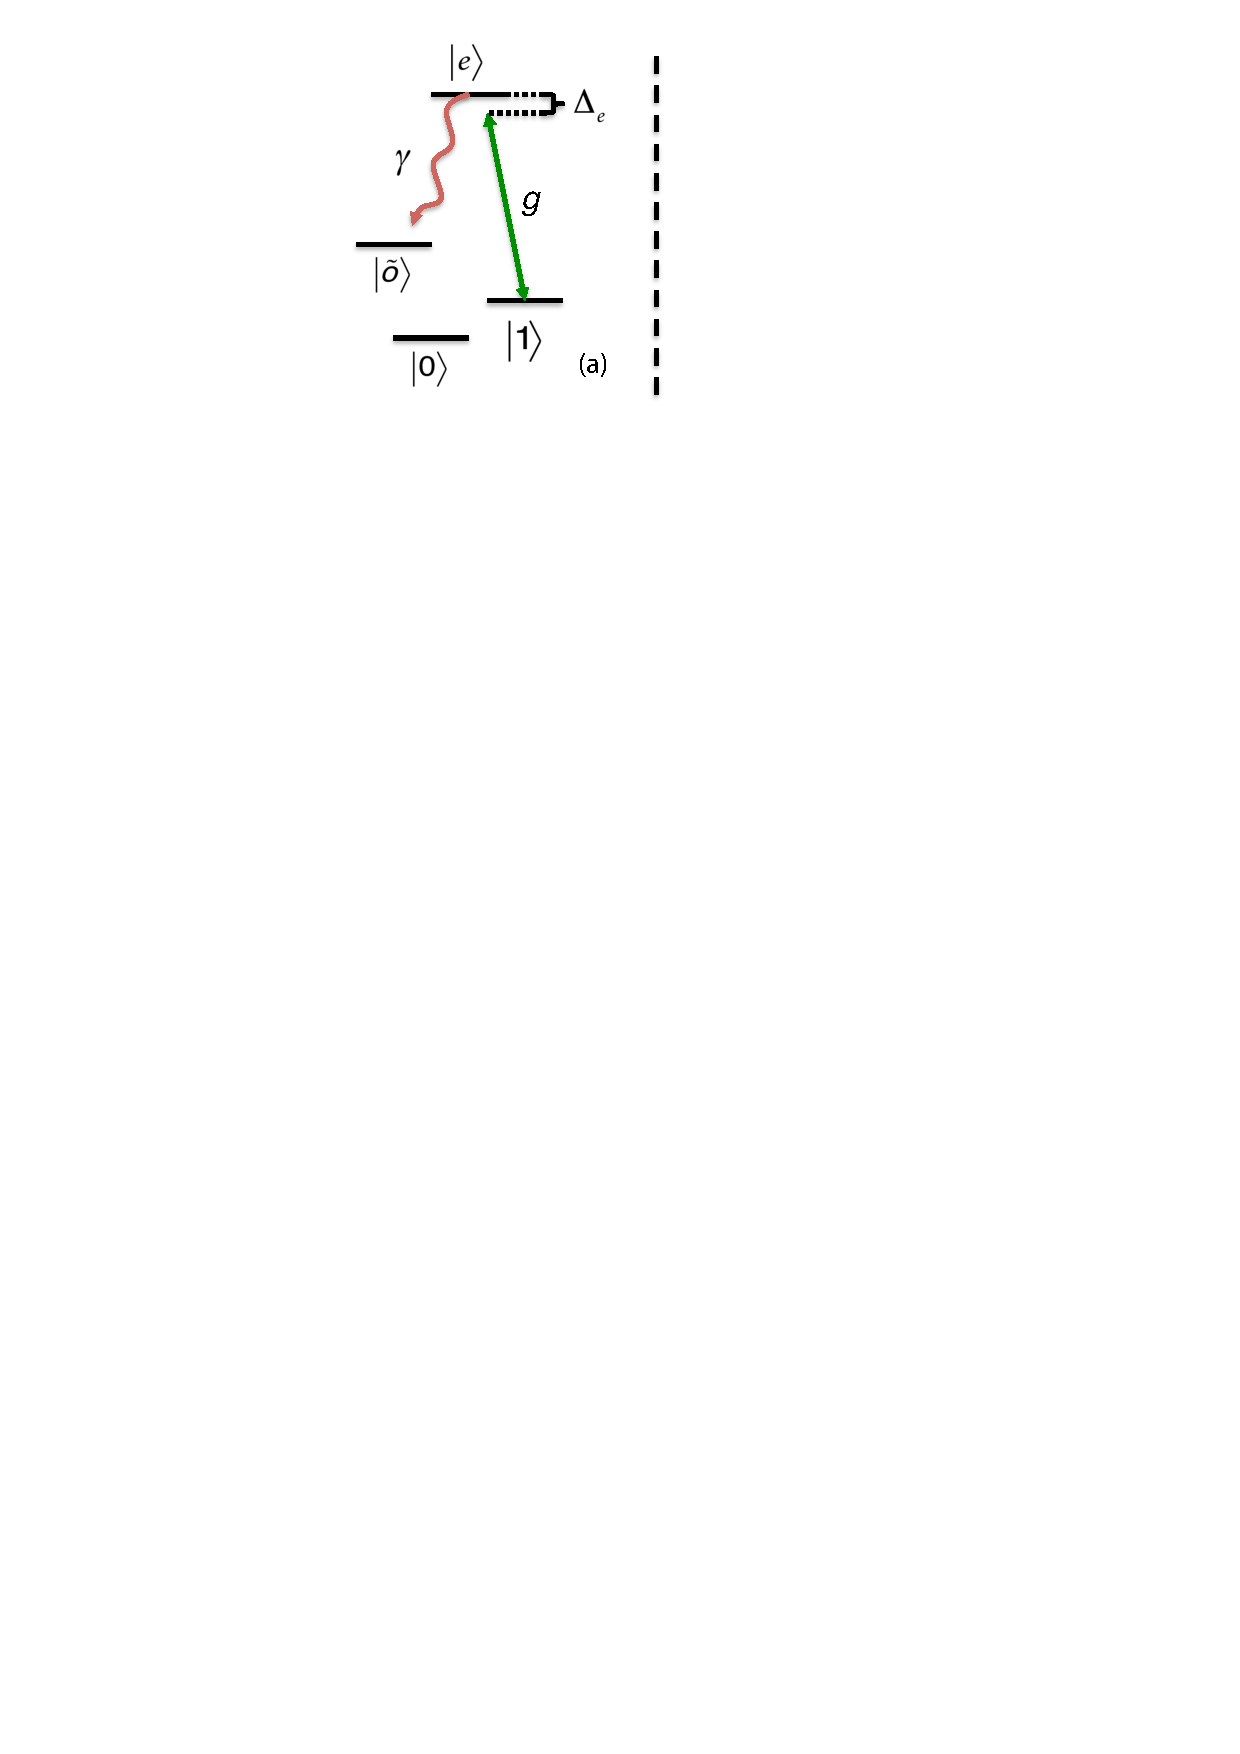
\includegraphics[width=0.35\textwidth]{./figs_Borregaard_PRL2015/figureS1a}
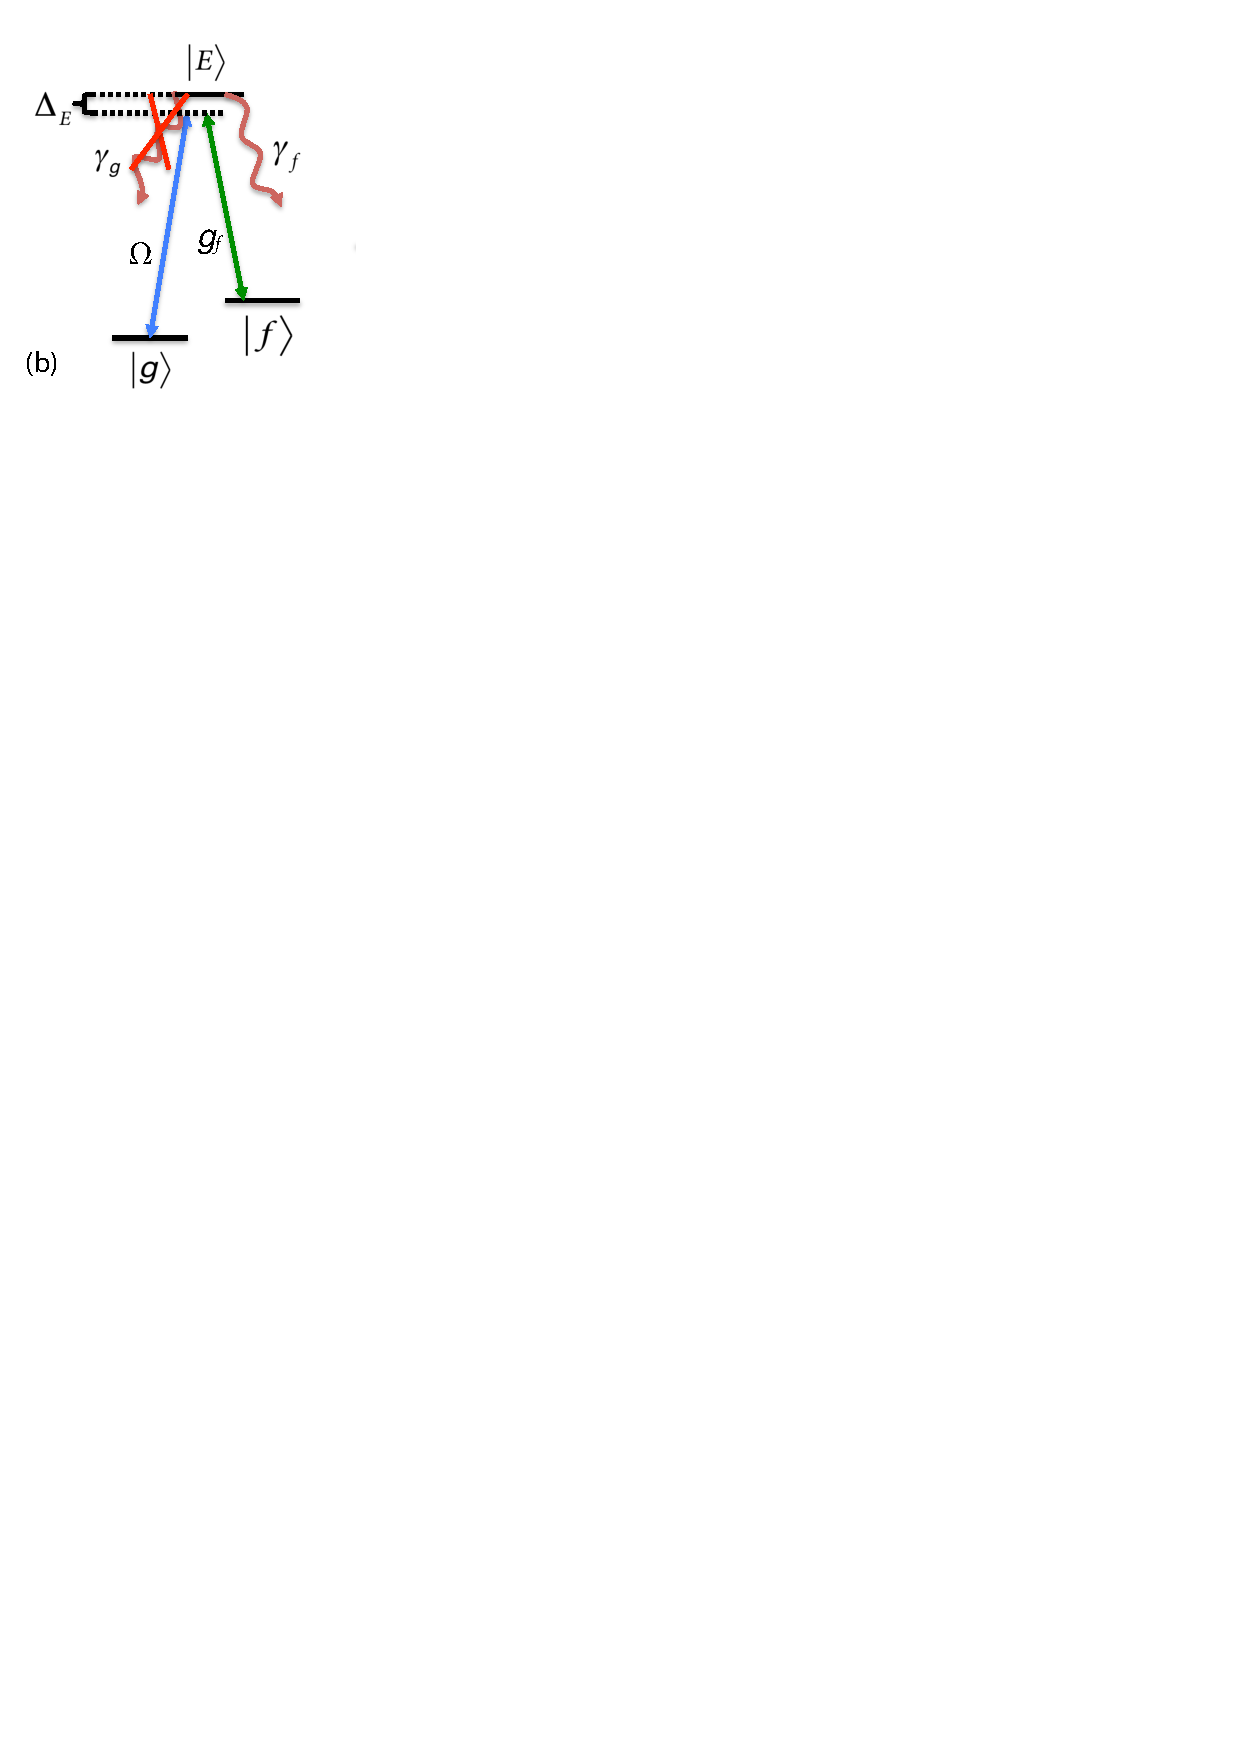
\includegraphics[width=0.35\textwidth]{./figs_Borregaard_PRL2015/figureS1b}
\caption
[Level structure of qubit an auxiliary atoms]
{(a) Level structure of the qubit atoms. Only state $\ket{1}$ couples
to the cavity and we assume that the excited level decays to some level
$\ket{\tilde{o}}$, possible identical to $\ket{f}$ or $\ket{0}$. (b) Level
structure of the auxiliary atom and the transitions driven by the weak laser
($\Omega$) and the cavity ($g_{f}$). We allow for some decay from
$\ket{E}\to\ket{g}$ with decay rate $\gamma_{g}$. }
\label{fig:figureS1}
\end{figure}

The Hamilton describing the system in a proper rotating frame is given by Eqs.
(1)-(3) in the article and is reproduced here
\begin{eqnarray} \label{eq:hamil1}
\hat{H}&=&\hat{H}_{e}+\hat{V}+\hat{V}^{\dagger}, \\
\hat{H}_{e}&=&\Delta_{E}\ket{E}\bra{E}+g_{f}(\hat{a}\ket{E}\bra{f}+H.c) \nonumber \\
&&+\sum_{k}\Delta_{e}\ket{e}_{k}\bra{e}+g(\hat{a}\ket{e}_{k}\bra{1}+H.c), \\
\hat{V}&=&\frac{\Omega}{2}\ket{E}\bra{g},
\end{eqnarray}          
where we have assumed for simplicty that all couplings ($g,\Omega$) are real and
$k$ labels the qubit atoms ($\hbar=1$). We have defined
$\Delta_{E}=\omega_{E}-\omega_{g}-\omega_{L}$, and
$\Delta_{e}=\omega_{e}-\omega_{g}-\omega_{L}+\omega_{f}-\omega_{1}$ where
$\omega_{L}$ is the laser frequency and otherwise $\omega_{x}$ is the frequency
associated with level $x$. Note that we assume the cavity frequency to be
$\omega_{c}=\omega_{L}+\omega_{g}-\omega_{f}$ such that we are on resonance with
the $\ket{g}\to\ket{E}\to\ket{f}$ two-photon transition.

The dissipation in the system is assumed to be described by Lindblad operators
such that $\hat{L}_{0}=\sqrt{\kappa}\hat{a}$ describes the cavity decay with
decay rate $\kappa$, $\hat{L}_{g}=\sqrt{\gamma_{g}}\ket{g}\bra{E}$, and
$\hat{L}_{f}=\sqrt{\gamma_{f}}\ket{f}\bra{E}$ describes the decay of the
auxiliary atom and $\hat{L}_{k}=\sqrt{\gamma}\ket{\tilde{o}}_{i}\bra{e}$
describes the decay of the qubit atoms ($k=1,2\ldots N$). As described in the
article $\ket{\tilde{o}}$ may or may not coincide with $\ket{0}$ or $\ket{1}$.
Assuming that $\Omega$ is weak ($\Omega^{2}/\Delta_{E}\ll\Delta_{E}$ and
$\Omega\ll g$), we can treat the driving as a perturbation to the system. As
shown in Ref.~\cite{Florentin}, the dynamics of the system is then governed by
an effective master equation of the form
\begin{equation}
\dot{\rho}=i\left[\rho,\hat{H}_{\text{eff}}\right] +
\sum_{x}\hat{L}_{x}^{\text{eff}}\rho(\hat{L}_{x}^{\text{eff}})^{\dagger}-\frac{1}{2}\left((\hat{L}_{x}^{\text{eff}})^{\dagger}\hat{L}_{x}^{\text{eff}}\rho+\rho(\hat{L}_{x}^{\text{eff}})^{\dagger}\hat{L}_{x}^{\text{eff}}\right),
\end{equation}
where $\rho$ is the density matrix of the system, $\hat{H}_{\text{eff}}$ is an
effective Hamiltonian, and  $L_{x}^{\text{eff}}$ are effective Lindblad
operators with $x=0,g,f,k$.  The effective operators are found from:
\begin{eqnarray} \label{eq:supheff1}
\hat{H}_{\text{eff}}&=&-\frac{1}{2}\hat{V}^{\dagger}\left(\hat{H}_{\text{NH}}^{-1}+(\hat{H}_{\text{NH}}^{-1})^{\dagger}\right)\hat{V}
\\
\hat{L}_{x}^{\text{eff}}&=&\hat{L}_{x}\hat{H}_{\text{NH}}^{-1}\hat{V},  \label{eq:supleff1}
\end{eqnarray}
where 
\begin{equation}
\hat{H}_{\text{NH}}=\hat{H}_{e}-\frac{i}{2}\sum_{x}\hat{L}_{x}^{\dagger}\hat{L}_{x},
\end{equation}
is the no-jump Hamiltonian. The Hilbert space of the effective operators can be
described in the basis of $\left\{\ket{g},\ket{f}\right\}$ of the auxiliary atom
and the states $\left\{\ket{0},\ket{1},\ket{\tilde{o}}\right\}$ of the qubit
atoms. To ease the notation, we define the projection operators $\hat{P}_{n}$
which projects on to the states with $n$ qubits in state $\ket{1}$. From
Eq.~\eqref{eq:supheff1} and \eqref{eq:supleff1} we then find:
\begin{eqnarray}
\hat{H}_{\text{eff}}&=&\sum_{n=0}^{N}\frac{-\Omega^{2}}{4\gamma}\mathrm{Re}\left\{\frac{i\tilde{\Delta}_{e}/2+nC}{\tilde{\Delta}_{e}(i\tilde{\Delta}_{E}/2+C_{f})+\tilde{\Delta}_{E}nC}\right\}\ket{g}\bra{g}\otimes \hat{P}_{n} \nonumber \\
&=&\sum_{n=0}^{N}\Delta_{n}\ket{g}\bra{g}\otimes \hat{P}_{n}
\label{eq:supham2}\\
\hat{L}_{0}^{\text{eff}}&=&\sum_{n=0}^{N}\frac{1}{2\sqrt{\gamma}}\frac{\sqrt{C_{f}}\tilde{\Delta}_{e}\Omega}{\tilde{\Delta}_{e}(i\tilde{\Delta}_{E}/2+C_{f})+n\tilde{\Delta}_{E}C}\ket{f}\bra{g}\otimes
\hat{P}_{n} \nonumber \\
&=&\sum_{n=0}^{N}r_{0,n}^{\text{eff}}\ket{f}\bra{g}\otimes \hat{P}_{n}
\label{eq:subleff1} \\
\hat{L}_{g}^{\text{eff}}&=&\sum_{n=0}^{N}\frac{1}{2}\frac{(i\tilde{\Delta}_{e}/2+nC)\Omega}{\tilde{\Delta}_{e}(i\tilde{\Delta}_{E}/2+C_{f})+n\tilde{\Delta}_{E}C}\frac{\sqrt{\gamma_{g}}}{\gamma}\ket{g}\bra{g}\otimes
\hat{P}_{n} \nonumber \\
&=&\sum_{n=0}^{N}r_{g,n}^{\text{eff}}\ket{g}\bra{g}\otimes \hat{P}_{n} \\
\hat{L}_{f}^{\text{eff}}&=&\sum_{n=0}^{N}\frac{1}{2}\frac{(i\tilde{\Delta}_{e}/2+nC)\Omega}{\tilde{\Delta}_{e}(i\tilde{\Delta}_{E}/2+C_{f})+n\tilde{\Delta}_{E}C}\frac{\sqrt{\gamma_{f}}}{\gamma}\ket{f}\bra{g}\otimes
\hat{P}_{n} \nonumber \\
&=&\sum_{n=0}^{N}r_{f,n}^{\text{eff}}\ket{f}\bra{g}\otimes \hat{P}_{n} \\
\hat{L}_{k}^{\text{eff}}&=&\sum_{n=1}^{N}-\frac{1}{2\sqrt{\gamma}}\frac{\sqrt{C_{f}}\sqrt{C}\Omega}{\tilde{\Delta}_{e}(i\tilde{\Delta}_{E}/2+C_{f})+n\tilde{\Delta}_{E}C}\ket{f}\bra{g}\otimes\ket{\tilde{o}}_{k}\bra{1}\otimes\hat{P}_{n}
\nonumber \\
&=&\sum_{n=1}^{N}r_{n}^{\text{eff}}\ket{f}\bra{g}\otimes\ket{\tilde{o}}_{k}\bra{1}\otimes\hat{P}_{n},
\label{eq:subleff2}
\end{eqnarray}
where we have defined the cooperativities $C_{(f)}=g_{(f)}^{2}/\gamma\kappa$ for
the qubit (auxiliary) atoms and the complex detunings
$\tilde{\Delta}_{E}\gamma=\Delta_{E}-i\gamma_{f}/2$ and 
$\tilde{\Delta}_{e}\gamma=\Delta_{e}-i\gamma/2$. Note that we have defined the
parameters $r^{\text{eff}}_{0,n}, r^{\text{eff}}_{g,n},r^{\text{eff}}_{f,n}$ and
$r_{n}^{\text{eff}}$ in Eqs. \eqref{eq:subleff1}-\eqref{eq:subleff2} to
characterize the decays described by the Lindblad operators. Note that
$r_{0}^{\text{eff}}=0$. In our calculations we parametrize the difference
between the auxiliary atom and the qubit atoms by $C_{f}=\alpha C$ and
$\gamma_{f}=\beta\gamma$ to easier treat the limit of $C\gg1$ that we are
interested in.

\subsection{Success probability and fidelity}
Eqs. \eqref{eq:subleff1}-\eqref{eq:subleff2} show that the effect of all
Lindblad operators, except $\hat{L}_{g}^{\text{eff}}$, is that the state of the
auxiliary atom is left in state $\ket{f}$. All these errors are thus detectable
by measuring the state of the auxiliary atom at the end of the gate. For the
heralded gates where we condition on measuring the auxiliary atom in state
$\ket{g}$ at the end of the gates, these detectable decays therefore do not
effect the fidelity of the gates but only the success probability.  The rate
$\Gamma_{n}$ of the detectable decays for a state with $n$ qubits in state
$\ket{1}$ is
$\Gamma_{n}=\abs{r_{0,n}^{\text{eff}}}^{2}+\abs{r_{f,n}^{\text{eff}}}^{2}+\abs{r_{n}^{\text{eff}}}^{2}$
and assuming an initial qubit state described by density matrix $\rho_{qubit}$
the success probability of the gates is
\begin{equation}
P_{\text{success}}=
\sum_{n=0}^{N}\text{Tr}
\left\{e^{-\Gamma_{n}t_{\text{gate}}}\rho_{\text{qubit}}\hat{P}_{n}\right\},
\end{equation}
where $t_{\text{gate}}$ is the gate time and $\text{Tr}$ denotes the trace. 

Having removed the detrimental effect of the detectable errors by heralding on a
measurement of the auxiliary atom the fidelity of the gates will be determined
by more subtle, undetectable errors (see below). We define the fidelity, $F$ of
the gate as
\begin{equation}
F=\frac{1}{P_{\text{success}}}\bra{\psi}\bra{g}
\tilde{\rho}_{\text{qubit}}\ket{g}\ket{\psi},
\end{equation} 
where we have assumed that the ideal qubit state after the gate is a pure state
$\ket{\psi}$ and $\tilde{\rho}_{qubit}$ is the actual density matrix of the
qubits and the auxiliary atom after the gate operation.

\subsection{$N$-qubit Toffoli gate}

As shown in the article, the effective Hamiltonian in Eq.~\eqref{eq:supham2} is
sufficient to make a Toffoli gate by putting the qubit atoms on resonance
($\Delta_{e}=0$). We will now treat the worst case and average fidelities of the
general Toffoli gate referred to in the article. The undetectable errors
limiting the fidelities are the following.
\begin{itemize}
\item As described in the article the energy shifts of the coupled qubit states
are all $\Delta_{n>0}\sim\Omega^{2}/(4\gamma\sqrt{C})$ in the limit $C\gg1$.
However, to higher order in $C$, we find corrections on the order
$\mathcal{O}(\Omega^{2}/C^{3/2})$ to the energy shifts, which depend on the
number of qubits that couples. The gate time of the Toffoli gate is
$t_{\text{T}}\sim4\pi\sqrt{C}\gamma/\Omega^{2}$ and consequently, the higher
order corrections give uneven phase shifts on the order of $\mathcal{O}(C^{-1})$
for the coupled qubit states at the end of the gate. This leads to a phase error
in the fidelity of $\mathcal{O}(C^{-2})$.
\item The difference between the rates of detectable errors ($\Gamma_{n}$) for
different qubit states changes the relative weight of the qubit states during
the gate. This error wil be $\mathcal{O}(C^{-1})$ as shown below.
\item For $\gamma_{g}>0$ the undetectable decay from $\ket{E}\to\ket{g}$ in the
auxiliary atom will destroy the coherence between the qubit states. We find that
this error will be $\sim \frac{\gamma_{g}}{\gamma\sqrt{C}}$. For now, we will
assume that $\gamma_{g}=0$ and thus ignore this error since we will show that we
can suppress the branching fraction $\gamma_{g}/\gamma$ arbitrary close to zero
by having a two photon driving.
\end{itemize}  

Assuming that $\gamma_{g}=0$, the dominating source of error limiting the
performance of the Toffoli gate is thus the difference between the rates of the
detectable errors for the qubit states. We tune $\Delta_{E}$ such that
$\Gamma_{0}=\Gamma_{1}$ and the largest difference between the detectable errors
is thus between the completely uncoupled state and the state with all qubit
atoms in state $\ket{1}$. As a result, we can find an upper bound on the
fidelity of the $N$ qubit Toffoli gate, considering an initial state
$\ket{0}^{\otimes N}+\ket{1}^{\otimes N}$ in the limit $N\to\infty$ because this
state experiences the largest difference between the number of coupled and
uncoupled qubits. We find that the upper bound on the fidelity and the
corresponding success probability is
\begin{eqnarray}
F_{\text{up}}&\sim&1-\frac{\pi^{2}\alpha}{16(\alpha+\beta)}\frac{1}{C}\\
P_{\text{success,up}}&\sim&1-
\frac{(\alpha+2\beta)\pi}{2\sqrt{\alpha}\sqrt{\alpha+\beta}} \frac{1}{\sqrt{C}}.
\end{eqnarray}.   
In general, the fidelity of the gate will, however, be larger than what is
suggested above. Considering a generic input state  $(\ket{0}+\ket{1})^{\otimes
N}$ with the same parameters as above, we find
\begin{eqnarray}
F_{\text{gen}}&\sim&1-k(N)\frac{\alpha \pi^{2}}{\alpha+\beta}\frac{1}{C} \\
P_{\text{success,gen}}&\sim&1-\frac{(d(N)\alpha+2\beta)\pi}{2\sqrt{\alpha}\sqrt{\alpha+\beta}}
\frac{1}{\sqrt{C}},
\end{eqnarray}
where $k(N),d(N)$ are scaling factors which depend on the number of qubits $N$.
We calculate $k(N)$ and $d(N)$ numerically for $N=1-100$ using the perturbation
theory and find that that they both decrease with $N$ (see
\reffig{fig:toffoli}). The upper bounded and generic fidelities and
corresponding success probabilities are shown in \reffig{fig:toffoli} for
different number of qubits, $N$.
\begin{figure} 
\centering
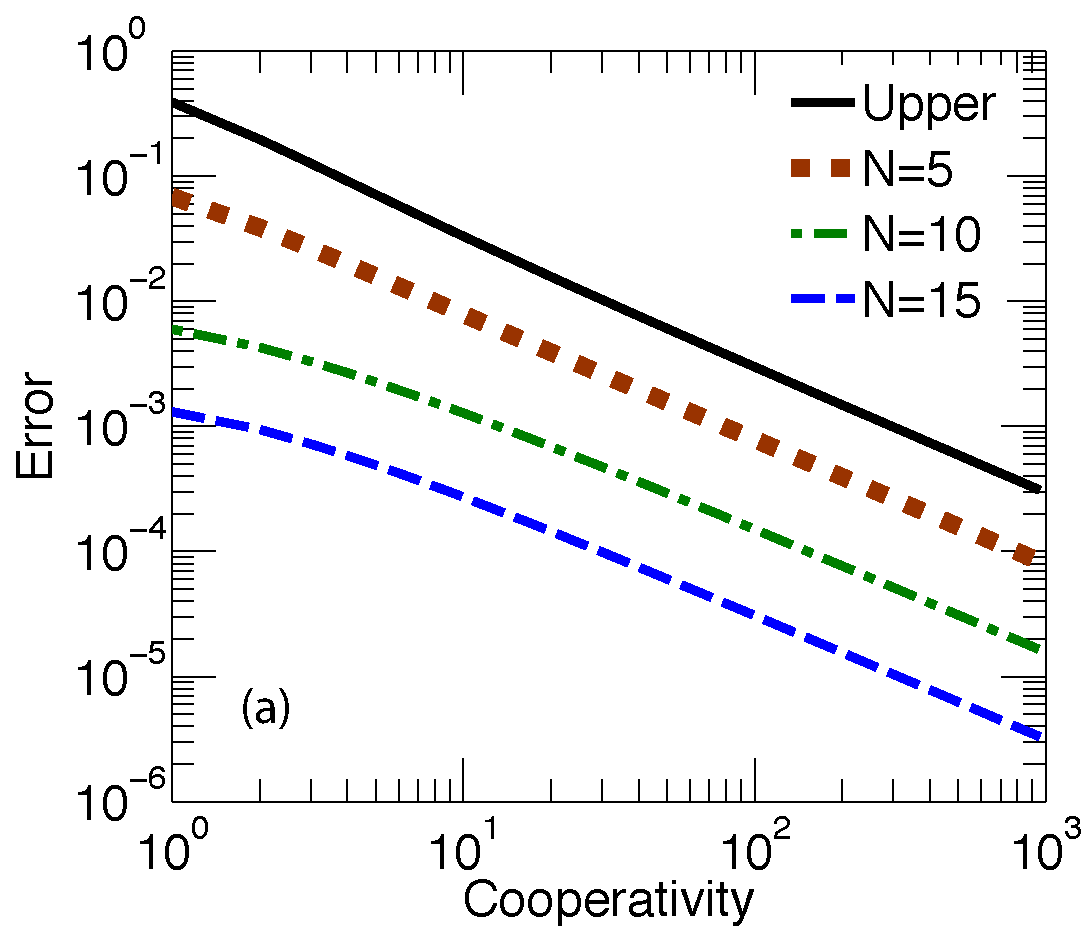
\includegraphics[width=0.46\textwidth]{./figs_Borregaard_PRL2015/figure2a}
\quad\quad
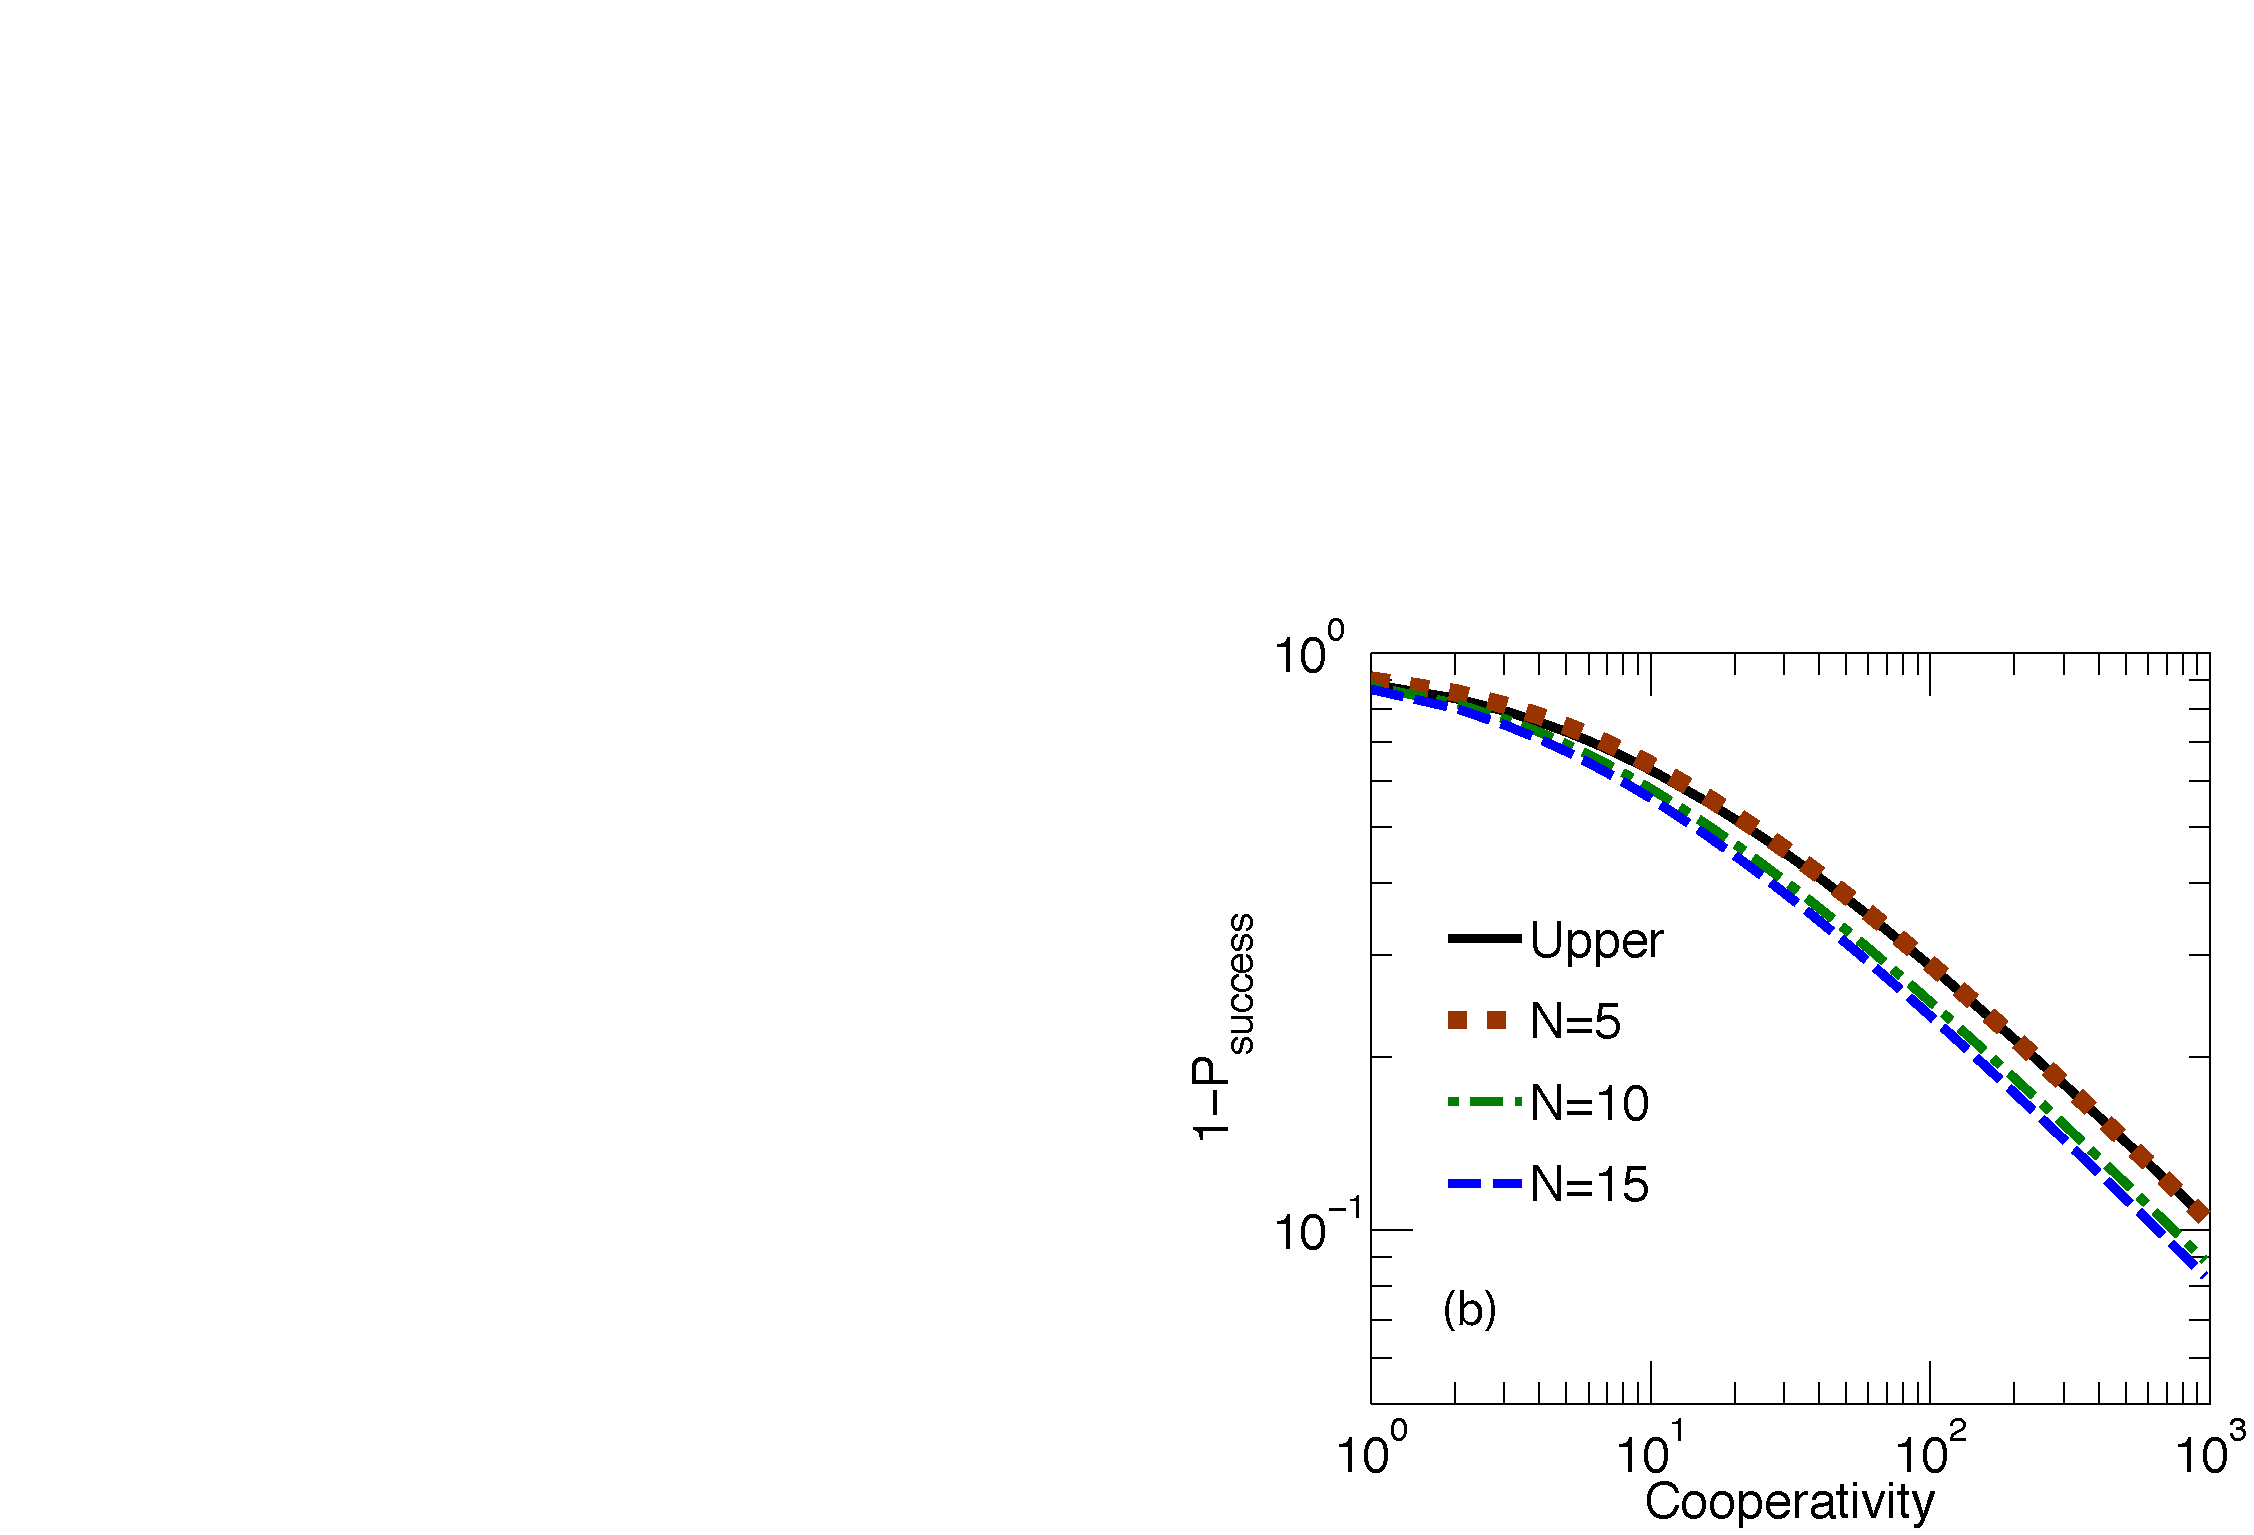
\includegraphics[width=0.46\textwidth]{./figs_Borregaard_PRL2015/figure2b}
\caption
[Error and success probability vs cooperativity]
{(a) Gate error of the Toffoli for different initial states as a
function of cooperativity. We have plotted the generic error for $N=5,10$, and 15 and the upper bound of the error. Note that the generic error decreases as $N$ increases. We have fixed $\Delta$ such that $\Gamma_{0}=\Gamma_{1}$ and have assumed that $\alpha=\beta=1$. (b) The failure probabilities $1-P_{\text{success,up}}$ and  $1-P_{\text{success,gen}}$ as a function of cooperativity. $1-P_{\text{success,gen}}$ is plotted for $N=5,10,15$. We have used the same assumptions as in (a). In general, the failure probability only have a weak dependence on $N$. Note that the line for $1-P_{\text{success, gen}},N=5$ coincides with  $1-P_{\text{success,up}}$.}
\label{fig:toffoli}
\end{figure}
As $N$ increases we obtain higher generic fidelity, whereas the success
probability is almost independent of $N$.

\subsection{CZ-gate}

In the special case of only two qubits the Toffoli gate is referred to as a
control-phase (CZ) gate. As shown in the article, we can, in this case,
completely remove the errors from the gate by choosing the detunings
$\Delta_{E}$ and $\Delta_{e}$ such that $\Gamma_{0}=\Gamma_{1}=\Gamma_{2}$ and
combining it with single qubit rotations we can ensure the right phase
evolution. In the general case where $\alpha,\beta\neq1$, the detunings
$\Delta_{e}$ and $\Delta_{E}$ are
\begin{eqnarray}
\Delta_{E}&=&\frac{\gamma}{2}\sqrt{\beta}\sqrt{4\alpha C+\beta} \\
\Delta_{e}&=&\frac{\alpha C\gamma^{2}}{2\Delta_{E}}. 
\end{eqnarray}
The success probability of the gate is then
\begin{equation}
P_{\text{success}}\simeq1-\pi\frac{8\beta^{2}+6\beta\alpha+\alpha^{2}}{8\beta^{3/2}\sqrt{\alpha}}\frac{1}{\sqrt{C}},
\end{equation} 
and we find that the gate time is
$t_{\text{CZ}}\simeq\frac{\gamma\pi\sqrt{\alpha}(\alpha+2\beta)(\alpha+4\beta)}{2\beta^{3/2}\Omega^{2}}\sqrt{C}$
in the limit $C\gg1$.
\subsection{Two-photon driving}

We now describe the details of the implementation where the auxiliary atoms is
driven by a two-photon process as shown in \reffig{fig:figureS2} (reproduced
from Fig. 4(a) in the article) in order to suppress the dominant undetectable
error caused by spontaneous decay of the auxilliary atom into the state
$\ket{g}$ ($\hat{L}_{g}$).

\begin{figure}
\centering
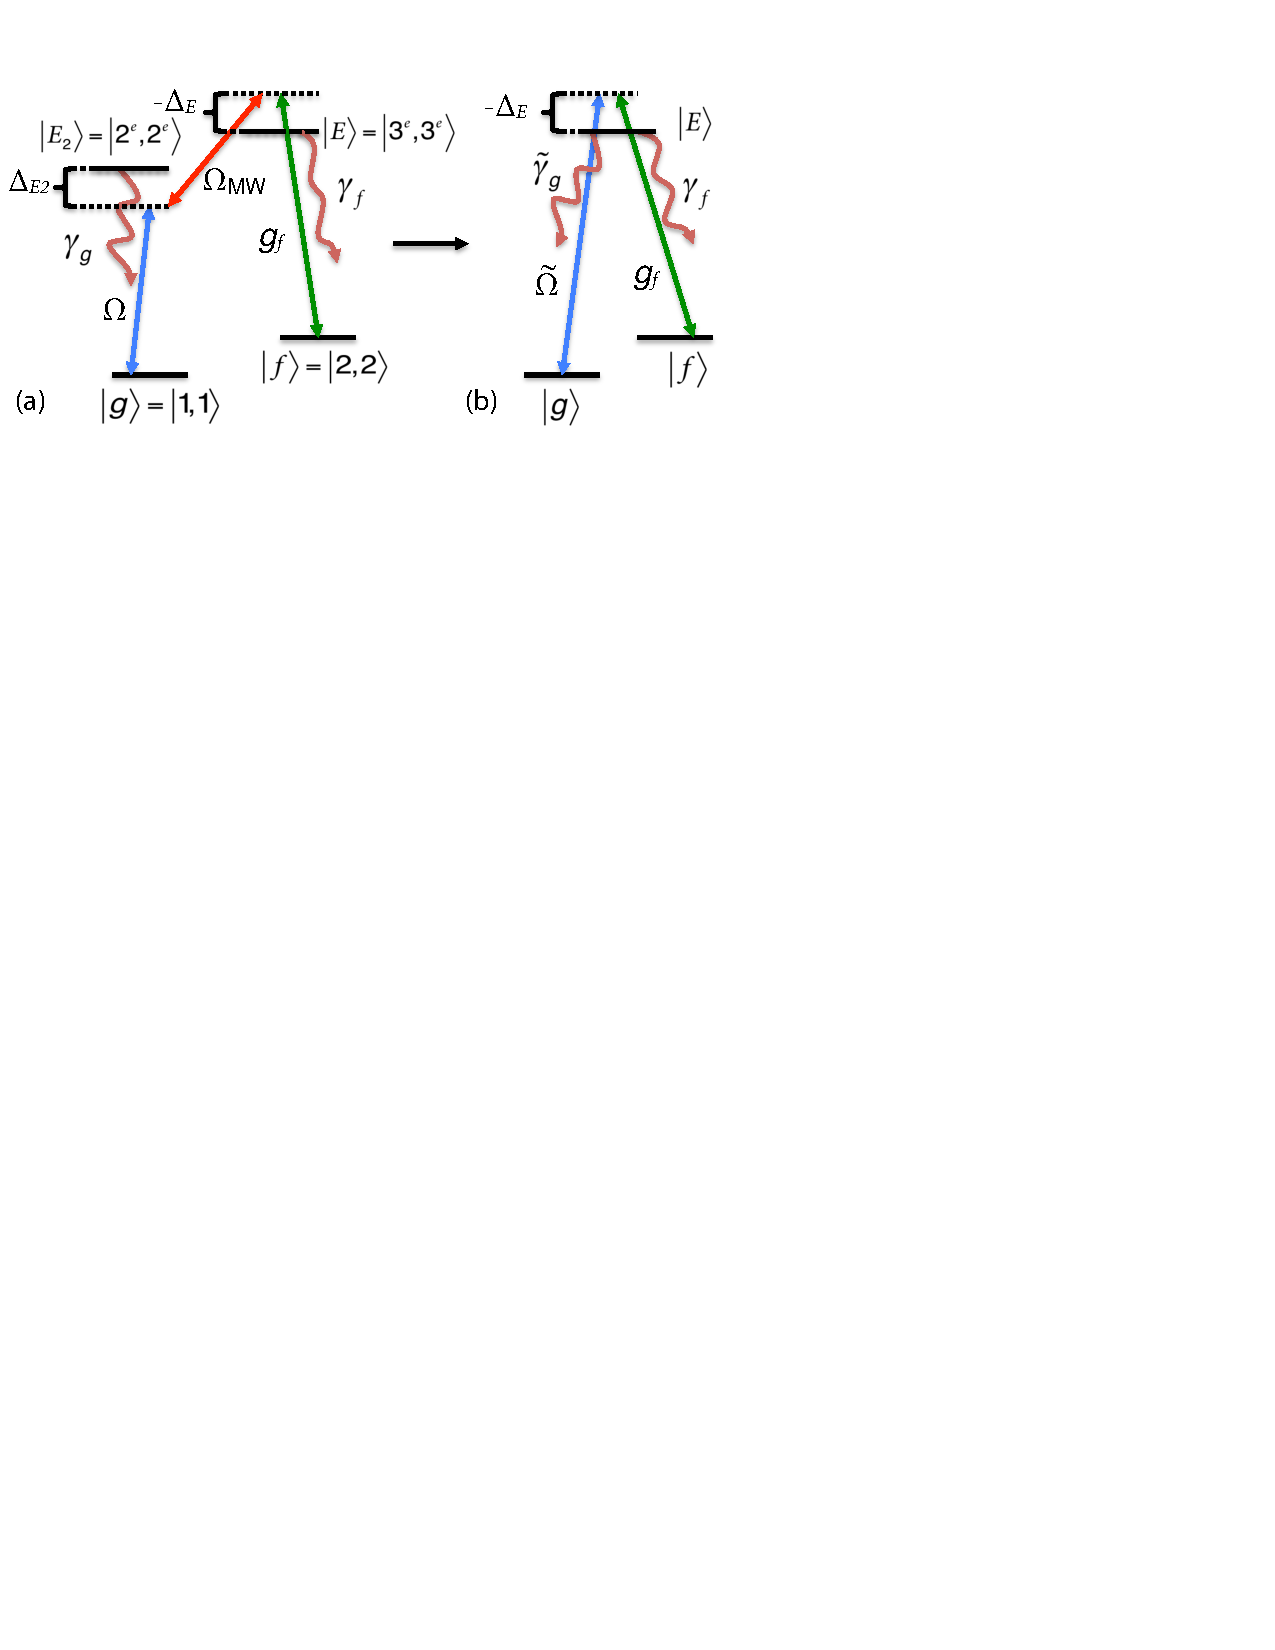
\includegraphics[width=0.7\textwidth]{./figs_Borregaard_PRL2015/figureS2} 
\caption
[Levels structure of auxiliary atom]
{(a) Level structure of the auxiliary atom and the transitions driven by
a weak laser ($\Omega$), a microwave field ($\Omega_{\text{MW}}$) and the cavity
($g_{f}$). We assume that $\ket{E}\leftrightarrow\ket{f}$ is a closed transition
and for simplicity we also assume that $\ket{E_{2}}\leftrightarrow\ket{g}$ is a
closed transition but this is not a necessity. The figure also indicates how the
levels could be realized in ${}^{87}$Rb. Here $\ket{r^{(e)},r^{(e)}}$ with
$r=1,2,3$ refers to state $\ket{\text{F}^{(e)}=r,\text{m}_{\text{F}}^{(e)}=r}$
in $5^{2}S_{1/2}$ $(5^{2}P_{3/2})$. (b) Effective three level atom realized by
mapping the two-photon drive to an effective decay rate $\tilde{\gamma}_{g}$ and
an effective drive $\tilde{\Omega}$}
\label{fig:figureS2}
\end{figure} 

The Hamiltonian in a proper rotating frame is
\begin{eqnarray} \label{eq:supphamil2}
\hat{H}&=&\hat{H}_{e}+\hat{V}+\hat{V}^{\dagger}, \\
\hat{H}_{e}&=&\Delta_{E}\ket{E}\bra{E}+\Delta_{E2}\ket{E_{2}}\bra{E_{2}}+g_{f}(\hat{a}\ket{E}\bra{f}+H.c)
\nonumber \\
&&+\frac{\Omega_{\text{MW}}}{2}(\ket{E}\bra{E_{2}}+H.c.) \nonumber \\
&&+\sum_{k}\Delta_{e}\ket{e}_{k}\bra{e}+g(\hat{a}\ket{e}_{k}\bra{1}+H.c.), \\
\hat{V}&=&\frac{\Omega}{2}\ket{E_{2}}\bra{g},
\end{eqnarray}  
where we have now defined
$\Delta_{E}=\omega_{E}-\omega_{g}-\omega_{laser}-\omega_{\text{MW}}$, 
$\Delta_{E2}=\omega_{E2}-\omega_{g}-\omega_{laser}$ and
$\Delta_{e}=\omega_{e}-\omega_{g}-\omega_{laser}-\omega_{\text{MW}}+\omega_{f}-\omega_{1}$.
Here $\omega_{laser}$ is the frequency of the laser drive ($\Omega$),
$\omega_{\text{MW}}$ is the frequency of the microwave field
($\Omega_{\text{MW}}$) and otherwise $\omega_{x}$ is the frequency associated
with level $x$. We assume that the frequency of the cavity is
$\omega_{c}=\omega_{laser}+\omega_{\text{MW}}+\omega_{g}-\omega_{f}$ such that
the three photon Raman transition from $\ket{g}\to\ket{f}$ is resonant. We have
assumed that $\Delta_{E2}$ is large and positive such that the rotating wave
approximation is valid for the microwave field.
The Lindblad operators describing the system are the same as described below
Eq.~\eqref{eq:hamil1} except that
$\hat{L}_{g}\to\sqrt{\gamma_{g}}\ket{g}\bra{E_{2}}$. Assuming a weak drive
$\Omega$, we can follow the same recipe as before to find the following
effective operators describing the dynamics of the system.
\bal
&&\hat{H}^{(2)}_{\text{eff}}
= \sum_{n=0}^{N}\Delta^{(2)}_{n}\ket{g}\bra{g} \otimes \hat{P}_{n}
\label{eq:supham3}\\
&&\qquad \Delta^{(2)}_{n} = \frac{-\Omega^{2}}{4\gamma}\mathrm{Re}
\left[\frac{\tilde{\Delta}_{e}(i\tilde{\Delta}_{E}/2+C_{f})+n
\tilde{\Delta}_{E}C}{\tilde{\Delta}_{E2}\tilde{\Delta}_{e}
(i\tilde{\Delta}_{E}/2+C_{f})+n\tilde{\Delta}_{E}\tilde{\Delta}_{E2}
C-i\tilde{\Delta}_{e}\tilde{\Omega}_{\text{MW}}^{2}/8-n
\tilde{\Omega}_{\text{MW}}^{2}C/4}\right]\nonumber
\\
&&\hat{L}_{0}^{\text{eff}(2)}=\sum_{n=0}^{N}r_{0,n}^{\text{eff}(2)}\ket{f}\bra{g}\otimes
\hat{P}_{n}
\label{eq:subleff3}\\
&&\qquad r_{0,n}^{\text{eff}(2)} =
\frac{-1}{4\sqrt{\gamma}}\frac{\sqrt{C_{f}}\tilde{\Delta}_{e}\Omega\tilde{\Omega}_{\text{MW}}}{\tilde{\Delta}_{E2}\tilde{\Delta}_{e}(i\tilde{\Delta}_{E}/2+C_{f})+n\tilde{\Delta}_{E2}\tilde{\Delta}_{E}C-i\tilde{\Delta}_{e}\tilde{\Omega}_{\text{MW}}^{2}/8-n\tilde{\Omega}_{\text{MW}}^{2}C/4}
\nonumber
\\
&&\hat{L}_{g}^{\text{eff}(2)}=\sum_{n=0}^{N}r_{g,n}^{\text{eff}(2)}\ket{g}\bra{g}\otimes
\hat{P}_{n}\\
&&\qquad r_{g,n}^{\text{eff}(2)} =
\frac{\Omega}{2}\frac{\tilde{\Delta}_{e}(i\tilde{\Delta}_{E}/2+C_{f})+n\tilde{\Delta}_{E}C}{\tilde{\Delta}_{E2}\tilde{\Delta}_{e}(i\tilde{\Delta}_{E}/2+C_{f})+n\tilde{\Delta}_{E2}\tilde{\Delta}_{E}C-i\tilde{\Delta}_{e}\tilde{\Omega}_{\text{MW}}^{2}/8-n\tilde{\Omega}_{\text{MW}}^{2}C/4}\frac{\sqrt{\gamma_{g}}}{\gamma}
\nonumber
\\
&&\hat{L}_{f}^{\text{eff}(2)} =
\sum_{n=0}^{N}r_{f,n}^{\text{eff}(2)}\ket{f}\bra{g} \otimes \hat{P}_{n}\\
&&\qquad r_{f,n}^{\text{eff}(2)} = 
-\frac{\Omega}{4}\frac{(i\tilde{\Delta}_{e}/2+nC)\tilde{\Omega}_{\text{MW}}}{\tilde{\Delta}_{E2}\tilde{\Delta}_{e}(i\tilde{\Delta}_{E}/2+C_{f})+n\tilde{\Delta}_{E2}\tilde{\Delta}_{E}C-i\tilde{\Delta}_{e}\tilde{\Omega}_{\text{MW}}^{2}/8-n\tilde{\Omega}_{\text{MW}}^{2}C/4}\frac{\sqrt{\gamma_{f}}}{\gamma}
\nonumber
\eal
\bal
&&\hat{L}_{k}^{\text{eff}(2)} =
\sum_{n=0}^{N-1}r_{n}^{\text{eff}(2)}\ket{f}\bra{g}\otimes\ket{\tilde{o}}_{k}\bra{1}\otimes
\hat{P}_{n}, \label{eq:subleff4} \\
&&\qquad r_{n}^{\text{eff}(2)} = 
\frac{1}{4\sqrt{\gamma}}\frac{\sqrt{C_{f}}\sqrt{C}\tilde{\Omega}_{\text{MW}}\Omega}{\tilde{\Delta}_{E2}\tilde{\Delta}_{e}(i\tilde{\Delta}_{E}/2+C_{f})+n\tilde{\Delta}_{E2}\tilde{\Delta}_{E}C-i\tilde{\Delta}_{e}\tilde{\Omega}_{\text{MW}}^{2}/8-n\tilde{\Omega}_{\text{MW}}^{2}C/4}
\nonumber
\eal
where we have defined the complex detuning
$\tilde{\Delta}_{E2}\gamma=\Delta_{E2}-i\gamma_{g}/2$ and the parameters
$r_{0,n}^{\text{eff}(2)},r_{g,n}^{\text{eff}(2)},r_{f,n}^{\text{eff}(2)}$ and
$r_{n}^{\text{eff}(2)}$ to characterize the decay described by the Lindblad
operators.

We are interested in the limit of large detuning $\Delta_{E2}$ and large
cooperativity $C$. In this limit, we find that the dynamics of the system can be
mapped to a simple three level atom with effective driving
$\tilde{\Omega}\sim\Omega\Omega_{\text{MW}}/(2\Delta_{E2})$ and an effective
decay $\tilde{\gamma}_{g}\sim\gamma_{g}\Omega_{\text{MW}}^{2}/\Delta_{E2}^{2}$
as shown in \reffig{fig:figureS2}. In principle, the effective operator
$\hat{L}_{0}^{\text{eff}(2)}$ leads to an effective decay rate of
$\tilde{\gamma}=\gamma_{g}\Omega^{2}/\Delta_{E2}^{2}$ to lowest order in $C$ 
but we find that this first order term do not destroy the coherence between the
qubit states since it is independent of $n$. There is, therefore, no effect of
these scattering events and the performance of the gate behaves as if there is
an effective decay rate of
$\tilde{\gamma}_{g}\sim\gamma_{g}\Omega_{\text{MW}}^{2}/\Delta_{E2}^{2}$. Note
that we also have an AC stark shift imposed on the level $\ket{g}$ by the laser
characterized by $\Omega$. This will give an overall phase to the system,
$\sim\Omega^{2}/(4\Delta_{E2})t$, which we can neglect since it does not
influence the gates.
Since we can do the mapping to the simple three level atom, we find similar
results for the performance of the gates for the two-photon scheme as for the
simple three level scheme only with effective decay $\tilde{\gamma}_{g}$ and
drive $\tilde{\Omega}$ given by the two-photon process. Note, however, that we
now assume $\gamma_{g}>0$, which introduces an undetectable error as previously
mentioned. We find that this introduces an error in the fidelity of both gates
of roughly
\begin{eqnarray}
&\sim&\frac{(\alpha^{2}-4\alpha\beta-6\beta^{2})\pi^{2}}{128\beta^{2}}\frac{\gamma_{g}^{4}}{\gamma^{4}\Delta_{E2}^{4}}+\frac{(\alpha^{2}+4\alpha\beta+6\beta^{2})\pi}{16\sqrt{\alpha\beta}(\alpha+2\beta)(\alpha+5\beta))}\frac{\gamma_{g}\Omega_{\text{MW}}^{2}}{\gamma\Delta_{E2}^{2}}\frac{1}{\sqrt{C}}\qquad.
\end{eqnarray}  
Nonetheless, this error can be suppressed arbitrarily much be increasing
$\Delta_{E2}$, which enable us to have a heralded CZ-gate with arbitrarily small
error in a realistic atomic setup using the two-photon drive.

\section{Gate time}
Here we address the question of how strongly we can drive the system and still
maintain the validity of perturbation theory. We need to adress this question
since the gate time depends inversely on the driving strength as shown in the
article and hence this limits the achievable gate time. A necessary criterion
for our pertubation theory to be valid is that the energy shifts $\Delta_{n}$
(see Eq.~\eqref{eq:supham2} and Eq.~\eqref{eq:supham3}) are small compared to
the driving, i.e. $\sim\Delta_{n}^{2}/\Omega^{2}\ll1$. From
Eq.~\eqref{eq:supham2} we find that
$\Delta_{n}^{2}/\Omega^{2}\sim\Omega^{2}/(16\Delta_{E}^{2})$ to leading order in
the cooperativity $C$ and this criterion is therefore met for
$\Omega\ll4\Delta_{E}$. Similarly, for the two-photon process, we find from
Eq.~\eqref{eq:supham3} that
$(\Delta_{n}^{(2)})^{2}/\Omega^{2}\sim\Omega^{2}/(16\Delta_{E2}^{2})$, to
leading order in $C$. Here we thus need $\Omega\ll4\Delta_{E2}$.

Another criterion need to be meet in order for our perturbative theory to be
valid. If none of the qubits couple, we are effectively driving the auxiliary
atom/cavity system into a dark state of the form
$\cos(\theta)\ket{0,g}-\sin(\theta)\ket{1,f}$, where the mixing angle is
$\theta\sim\Omega/g$. Here the number refers to the number of cavity photons. To
adiabatically eliminate the state $\ket{f,1}$ from the Hamiltonian as we have
done in the effective Hamiltonian requires that $\Omega/g\ll1$. Mapping this
criterion to the effective three level scheme realized in the two-photon scheme
gives $\Omega\Omega_{\text{MW}}/(2\Delta_{E2}g)\ll1$.

Finally, we need to consider the scattering of photons from the level $\ket{E2}$
in the two-photon scheme. If the number of scattering events, $n_{scat}$ is
large compared to $\Omega^{2}/(16\Delta_{E2}^{2})$, the perturbation theory is
not valid even though the other criterions are met. We find that
$n_{scat}\sim\frac{12\sqrt{C}\gamma^{2}}{\Omega_{\text{MW}}^{2}}$ for the
CZ-gate and we thus need to have 
$\frac{3\sqrt{C}\gamma^{2}\Omega^{2}}{\Delta_{E2}^{2}\Omega_{\text{MW}}^{2}}\ll1$

The different criterions for the validity of the perturbation theory are
summarized in \tabref{tab:tableS1}.
\begin{table} [H]
\centering
\begin{tabular}{|c|c|}
\hline
Simple scheme & Two-photon scheme  \\ \hline
$\Omega/(4\Delta_{E})\ll1$ & $\Omega/(4\Delta_{E2})\ll1$ \\ \hline
$\Omega/g\ll1$ & $\Omega\Omega_{\text{MW}}/(\Delta_{E2}g)\ll1$ \\ \hline
- & $3\sqrt{C}\gamma^{2}\Omega^{2}/(\Delta_{E2}^{2}\Omega_{\text{MW}}^{2})\ll1$  \\ \hline
\end{tabular}
\caption
[Perturbation validity criteria]
{The criterions for our perturbation theory to be valid. }
\label{tab:tableS1}
\end{table}
For all the gate schemes, we have assumed that
$\Delta_{E}\propto\sqrt{C}\gamma$. The first criterion for the simple scheme
(see \tabref{tab:tableS1}) can thus be met with a driving of
$\Omega=a\gamma\sqrt{C}$ where $a/4\ll1$. This driving results in a gate time
that decreases as $1/\sqrt{C}$. The value of $a$ will determine the size of the
non-adiabatic error. The second criterion is also fulfilled for this driving as
long as $\sqrt{\gamma/\kappa}\ll1$. In realistic systems such as the nanocavity
system described in Ref.~\cite{thompson, Tiecke}, the ratio $\kappa/\gamma$ can
be on the order of 100-1000.
For the two-photon scheme, we find from \tabref{tab:tableS1} that we can choose
$\Omega=a_{2}\Delta_{E2}, \Omega_{\text{MW}}=b\gamma C^{1/4}$ where the
constants $a_{2},b$ will determine the size of the non-adiabatic errors as
before. Similar to the situation in the simple scheme we assume that
$\sqrt{\gamma/\kappa}\ll1$.

\section{Numerical simulation}
In order to confirm our results, we numerically integrated the full Master
equation, defined by the Hamiltonian $\hat H$ and the Lindblad operators,
$\hat L_j \in \{\hat L_0, \hat L_g, \hat L_f, \hat L_1, \hat L_2\}$, 
\bel
\label{eq:full Master eq}
	\frac{d}{dt}\rho(t) = -\frac{i}{\hbar}[\hat H,\rho(t)]+\sum_j \frac{1}{2}
	\left[2 \hat L_j \rho(t) \hat L_j^{\dag} - \rho(t) \hat L_j^{\dag} \hat L_j -
	\hat L_j^{\dag} \hat L_j \rho(t)\right]
\eel
We used the QuTiP 2
package \cite{Johansson20131234}, for Python, to set up the problem and used its
12th-order numerical integration algorithm to find the solution $\rho(t)$ as a
time series.
Then, we used the routines of the same package to analyze the results. 

For each time series $\rho(t)$, we determined the gate time $t_{\text{gate}}$,
the success probability $P_{\text{success}}$, and the fidelity $F$.
We picked $\ket{\psi_0}_{12} =
\frac{1}{\sqrt{2}}\big(\ket{0} +
\ket{1}\big)_1\otimes\frac{1}{\sqrt{2}}\big(\ket{0}+ \ket{1}\big)_2$ as the
initial state of the two qubits, $\ket{g}$ for the control atom, and zero
photons in the cavity. Starting from here, we let the system evolve under the
Master equation Eq.~(\ref{eq:full Master eq}), and determined $P_g(t)$, the
conditional state $\rho_g(t)$ and $F(t)$ as a function of time:
\bal
	P_g(t) &=& \text{Tr}	\Big[\rho(t)\ket{g}\bra{g}\Big],
	\\
	\rho_g(t) &=& \frac{\ket{g}\bra{g}\rho(t)
	\ket{g}\bra{g}}{P_g(t)},
	\\
	F(t) &=& \max_{\phi_1, \phi_2}\Ev{\left.\psi_t^{\phi_1, \phi_2}\right|
	\text{Tr}_{\text{c, c}}\big(\rho_g(t)\big) \left| \psi_t^{\phi_1,
	\phi_2}\right.}
% 	E(t) &=& \text{Ent}\big(\;P_{\text{logical}}\;
% 	\text{Tr}_\text{control, cav}\big(\rho_g(t)\big)\;P_{\text{logical}}
% 	/\mathcal{N}\;\big),
\eal
where $\text{Tr}_{\text{c, c}}$ is the partial trace operation over
the control atom and the cavity, and $\ket{\psi_t^{\phi_1, \phi2}}$ is the
target state transformed with two single qubit $z$-rotations:
\bel
	\Ket{\psi_t^{\phi_1, \phi_2}} = \hat U_1(\phi_1) \hat U_2(\phi_2)
	\frac{1}{2}\Big(\ket{00} + \ket{01} + \ket{10} - \ket{11}\Big),
\eel
where $\hat U_{k}(\phi_k) = \exp\left[i \ket{1}_k\bra{1}_k \phi_k\right]$ is the
$z$-rotation of qubit $k$ ($= 1,2$) by the angle $\phi_k$.
% $P_\text{logical} =
% \ket{00}\bra{00} + \ket{01}\bra{01} + \ket{10}\bra{10} + \ket{11}\bra{11}$
% is the projector onto the logical subspace of the qubits, and $\mathcal{N}$ is a
% normalization constant.
% $\text{Ent}(\rho)$ of a two-qubit density matrix $\rho$
% is defined, according to \cite{Wootters1998}, as
% $
% 	\text{Ent}(\rho) = h\Big[\Big(1 + \sqrt{1-c^2(\rho)}\Big) /2\Big],
% $
% where $h(x) = -x\log_2 (x) - (1-x)\log_2(1-x)$, and $c(\rho)$ is the
% concurrence of $\rho$. We then determined the gate time $t_\text{gate}$ by
% finding the timepoint where $E(t)$ is maximal. 
From these time series, we determined the gate time $t_{\text{gate}}$ by
finding the timepoint where $F(t)$ is maximal,
\bel
	t_{\text{gate}} = \underset{t}{\text{argmax}}\;F(t)
\eel
 The fidelity and the success
probability of the gate is then defined as $F = F(t_{\text{gate}})$,
$P_{\text{success}} = P_g(t_{\text{gate}})$. 
% We chose to evaluate the fidelity
% through entanglement $E$, since it can be determined without the knowledge of
% the exact single-qubit rotations required to complete the gate, which are
% always easier to perform than two-qubit operations.

Plots of Fig.~\ref{fig:t_gate,P_success} show the gate time ($t_{\text{gate}}$)
and the success probability ($P_{\text{success}}$) as a function of $a$, for
$\gamma_g = 0$, $\gamma = 0.01\kappa$, $\Omega=a\gamma\sqrt{C}$ with
$C\in\{10,30,100,300,1000\}$. The detunings, $\Delta_E$ and $\Delta_e$ were
chosen to be close to their optimal value, determined from the adiabatic theory,
and numerically optimized to result in identical effective $\ket{g}\rightarrow
\ket{f}$ transition rates  $\Gamma_0 = \Gamma_1 = \Gamma_2$ for the qubit
sectors $\ket{00}, \ket{01}, \ket{11}$. The rates $\Gamma_j$ were found by
numerically diagonalizing the master equation for the qubit sectors separately,
and finding the eigenvalue with the smallest (but non-zero) absolute real part.
This numerical optimization yielded the maximal fidelity. The symbols correspond
to the numerical result, whereas the solid lines show the theoretical values.
The agreement of the results confirms the validity of the adiabatic theory for a
driving $\Omega=a\gamma\sqrt{C}$ for $C\lesssim 1000$ and $a\lesssim0.25$. Note,
however, that Fig.~\ref{fig:t_gate,P_success} shows how the success probability
deviates from the adiabatic result for $a\gtrsim0.25$. A weak increase of this
deviation with the cooperativity is seen but from simulations at high C, we
believe that this can be removed by gradually ramping $\Omega$ up and down to
maintain adiabaticity at the beginning and end of the driving pulse. This was
not included in the simulations behind Fig.~\ref{fig:t_gate,P_success} for
simplicity.
 \begin{figure}[h]
\centering
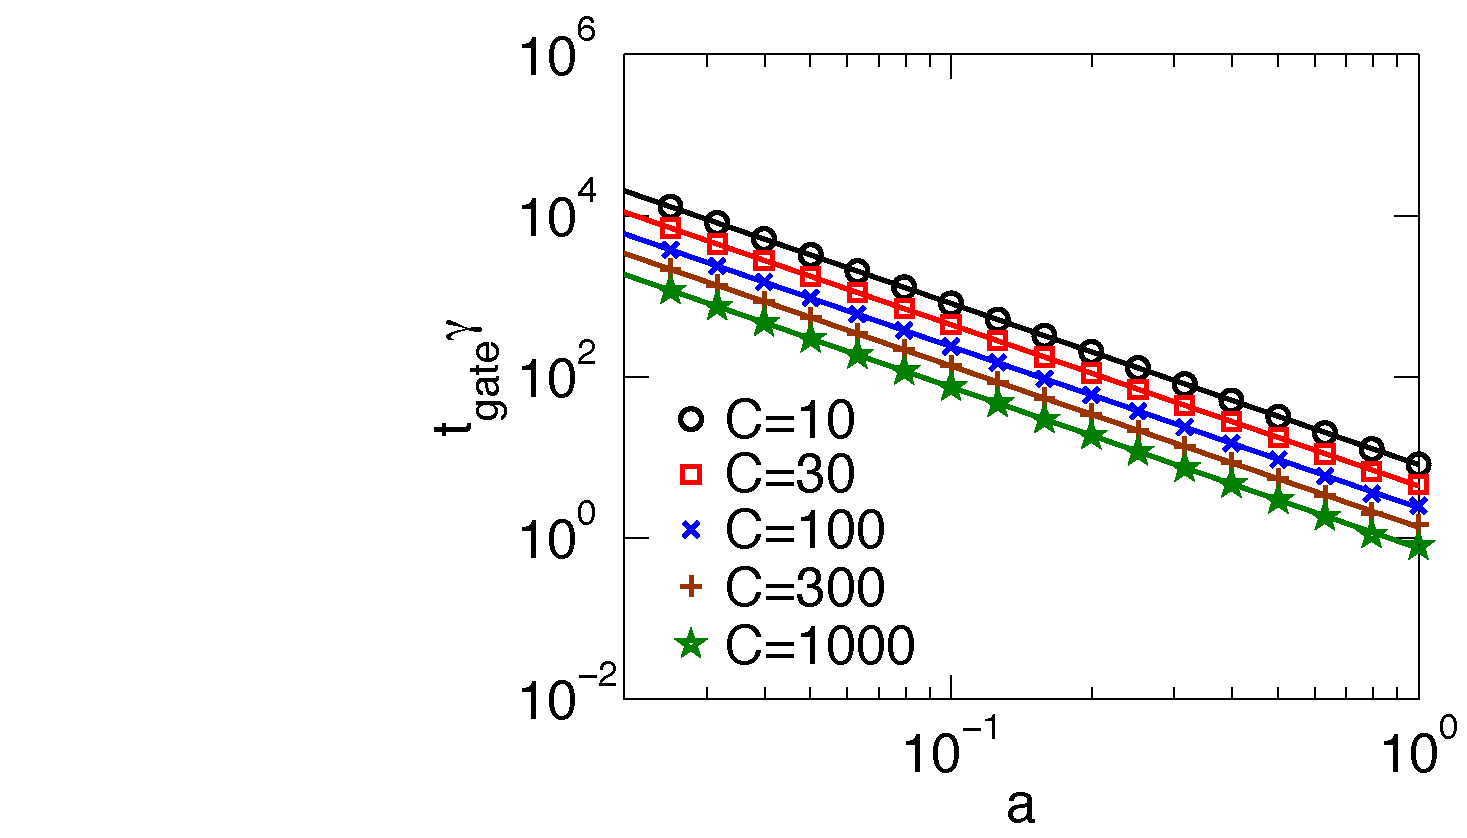
\includegraphics[width=0.48\textwidth]{./figs_Borregaard_PRL2015/figureSN1}\quad 
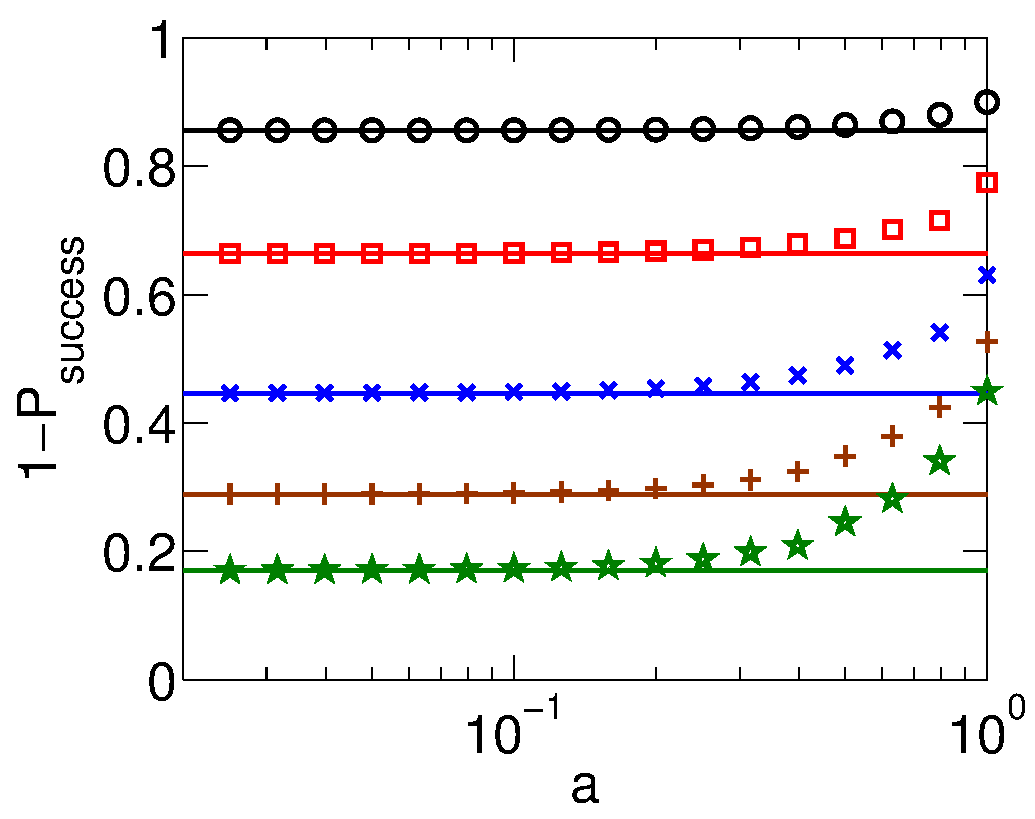
\includegraphics[width=0.48\textwidth]{./figs_Borregaard_PRL2015/figureSN2}
\caption
[Gate time and success probability vs driving strength]
{
\label{fig:t_gate,P_success}
Gate time (left) and failure probability (right) as a function of driving
strength ($a$) for $\gamma/\kappa = 0.01$, $\gamma_g = 0$, and
$C\in\{10,30,100,300,1000\}$. The driving strength was assumed to be
$\Omega=a\gamma\sqrt{C}$.}
\end{figure} 
 
Fig.~\ref{fig:F} shows the conditional \emph{in}fidelity of the gate as a
function of $a$ for the same parameters. The simulation confirms that using $a =
0.25$ is enough to push the (conditional) infidelity of the gate below
$4\cdot10^{-5}$. The fidelity is limited by non-adiabatic effects, which can be
suppressed by decreasing $\Omega$ as shown in the figure. Adiabatically ramping
Ω up and down at the beginning and end of the gate will also improve the
adiabaticity but, for simplicity, we have not included this in the simulations
described here. Note, however that for high $C$ ($C>1000$), we find that this
gradual ramping of $\Omega$ significantly decreases the non-adiabatic error.
\begin{figure}[h] 
\centering
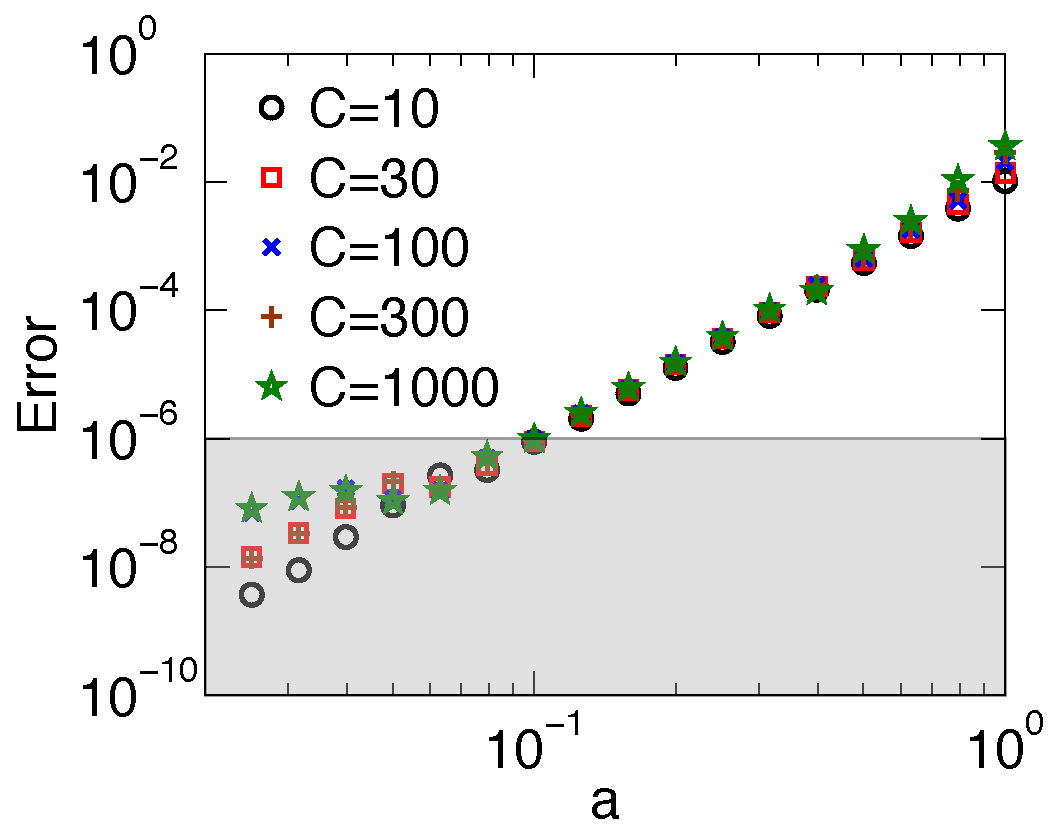
\includegraphics[width=0.5\textwidth]{./figs_Borregaard_PRL2015/figureSN3} 
\caption
[Conditional fidelity]
{ 
\label{fig:F}
Conditional infidelity of the gate as a function of the driving strength $(a)$
for $\gamma/\kappa = 0.01$, $\gamma_g = 0$, and $C\in\{10,30,100,300,1000\}$.
The shaded region (at $\sim 10^{-6}$) shows the limit of numerical accuracy. The
driving strength was assumed to be $\Omega=a\gamma\sqrt{C}$.}
\end{figure} 

We repeated the above analysis for the two-photon-driving Hamiltonian in
Eq.~\eqref{eq:supphamil2}. We chose $ \gamma = \gamma_g = \gamma_f =
0.01\,\kappa$,  $\Omega = \frac{\Delta_{E2}}{8 C^{1/4}}$, and
$\Omega_{\text{MW}} = 4\gamma C^{1/4}$, and chose $\Delta_E$ and $\Delta_e$
detunings again close to their adiabatic optimum, but numerically optimized them
with the same procedure as previously.
Plots of Fig.\ref{fig:t,P 2} show the gate time and the success probability as a
function of $\Delta_{E2}$ for $C\in\{10, 20, 50,100\}$. Symbols indicate the
numerical results while solid lines show the theoretical values.
 \begin{figure}[h]
\centering
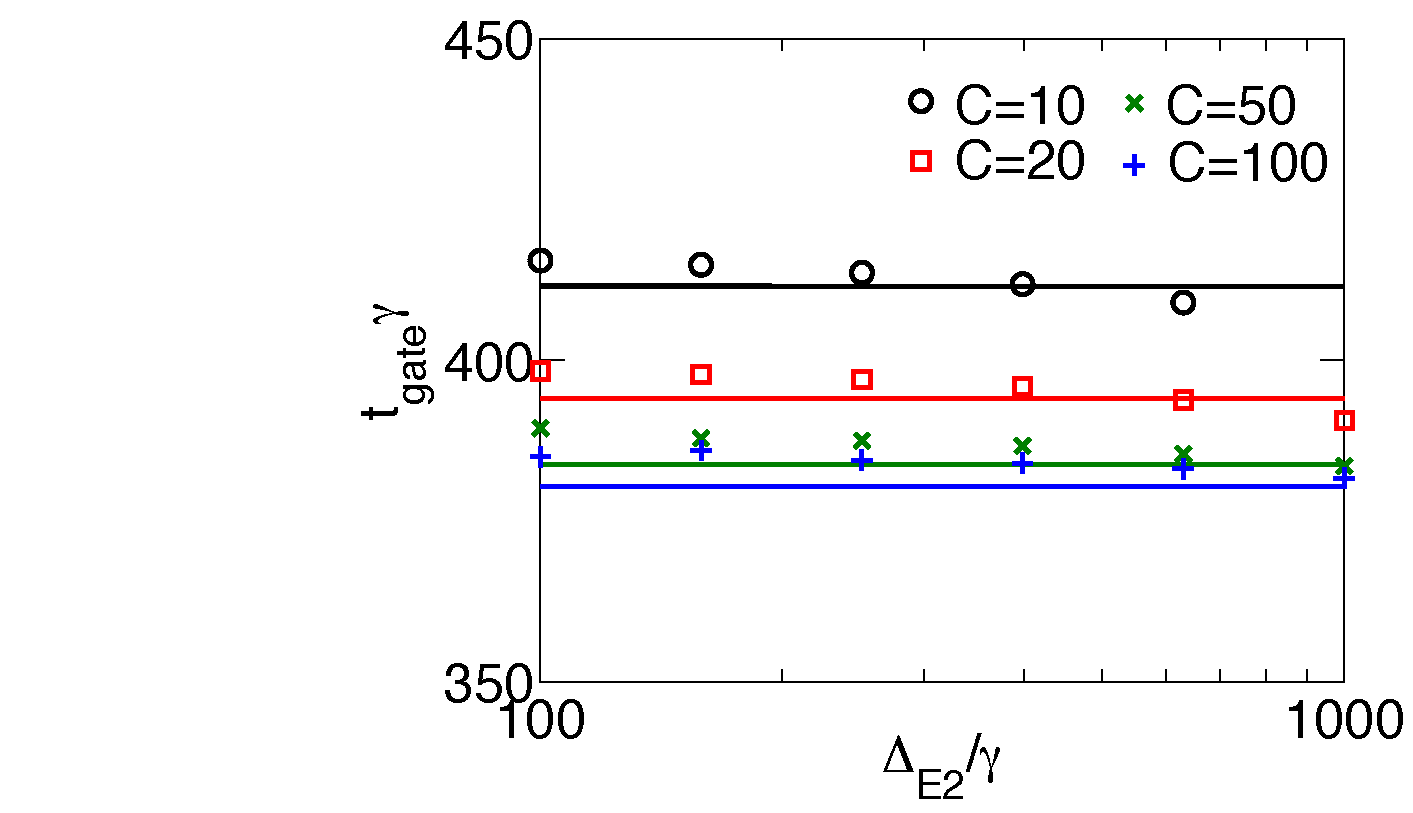
\includegraphics[width=0.48\textwidth]{./figs_Borregaard_PRL2015/figureSN4}\quad 
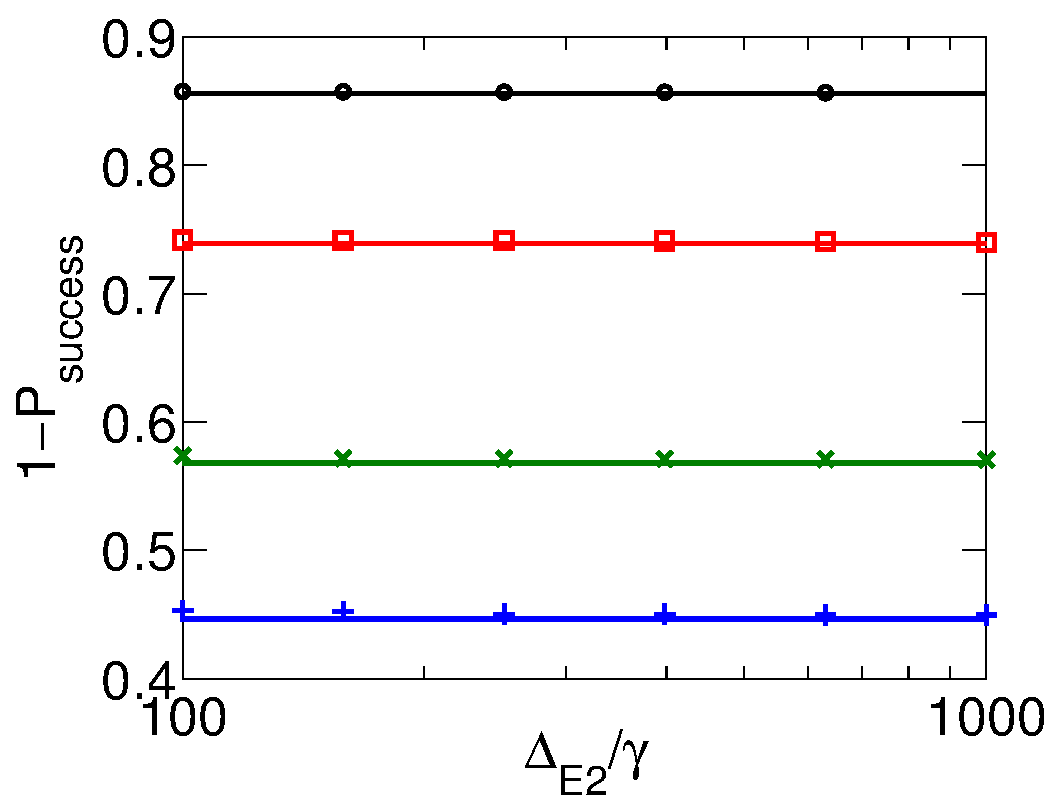
\includegraphics[width=0.48\textwidth]{./figs_Borregaard_PRL2015/figureSN5}
\caption
[Gate time and success probability vs detuning]
{
\label{fig:t,P 2} 
Gate time (left) and failure probability (right) as a function of $\Delta_{E2}$
for $\gamma = \gamma_g = \gamma_f = 0.01\kappa$, $\Omega = \frac{\Delta_{E2}}{8
C^{1/4}}$, $\Omega_{\text{MW}} = 4\gamma C^{1/4}$, $C = \{10,20,50,100\}$.
	}
\end{figure} 
Fig.~2b in the article shows the conditional \emph{in}fidelity of the
two-photon-driven gate as a function of $C$ for the same choice of parameters.
With these results, we confirm that by increasing $\Delta_{E2}$ we can lower the
infidelity error to an arbitrary small level. The gate time is a constant of the
cooperativity since we have increased $\Omega_{MW}$ as $C^{1/4}$ in the
simulations. We do see some deviation from the analytical results due to
non-adiabatic effects, which could be suppressed by decreasing $\Omega$ at the
expense of an increase in the gate time. Finally a gradual ramping of $\Omega$
could also decrease the non-adiabatic errors but for simplicity, we have not
included this in the simulations.

\section{Additional errors} 

There are some additional errors in a realistic atomic setup that we have not
treated in detail so far. Here we estimate the dominant errors and determine
under which conditions, they can be sufficiently suppressed such that they do
not limit the performance of the gates. We assume a realistic atomic setup where
${}^{87}$Rb atoms are used both for the auxiliary atom and the qubit atoms. In
the ${}^{87}$Rb atoms, we assume that $\ket{g}=\ket{1,1}, \ket{f}=\ket{2,2}$ and
$\ket{E_{2}}=\ket{2^{e},2^{e}}, \ket{E}=\ket{3^{e},3^{e}}$ where
$\ket{r^{(e)},r^{(e)}}$ with $r=1,2,3$ refers to state
$\ket{\text{F}^{(e)}=r,\text{m}_{\text{F}}^{(e)}=r}$ in $5^{2}S_{1/2}$
$(5^{2}P_{3/2})$. In this case, we estimate that the dominant errors are:
\begin{itemize}
\item In our perturbative theory, we have assumed that the laser field ($\Omega$) only couple $\ket{g}\to\ket{E2}$ in the auxiliary atom. However, for a large detuning $\Delta_{E2}$ it may also couple $\ket{f}\to\ket{E}$, which could lead to an undetectable error where the auxiliary atom is pumped back to $\ket{E2}$ from, which it decays to $\ket{g}$. This error is, however, suppressed by the large frequency separation, $\Delta_{g}$ of $\ket{g}$ and $\ket{f}$, which is $\Delta_{g}\sim1000\gamma$ for ${}^{87}$ Rb. We estimate the error using effective operators to find the decay rate back to $\ket{g}$, assuming that the auxiliary atom starts in $\ket{E2}$ and treating the drive $\Omega$ as a perturbation while neglecting the cavity coupling. This is valid as long as $\Delta_{g}\gg\Delta_{E}$, which is fulfilled for $C\lesssim10000$ since $\Delta_{E}\sim\sqrt{C}$. The error increases with $\Delta_{E2}$ but even for $\Delta_{E2}\approx400\gamma$ we find that for $\Omega_{\text{MW}}=4\gamma C^{1/4}$, $\Omega=\Delta_{E2}/8$ the error is $\lesssim10^{-4}$.     

\item The microwave might also couple the ground states $\ket{0}-\ket{1}$ of the
qubit atoms and the ground states $\ket{g}-\ket{f}$ of the auxiliary atom. The
coupling of $\ket{0}-\ket{1}$ means that the qubit atoms also couple to the
cavity even though they are in state $\ket{0}$. We estimate the error from this
to be on the order of
$\Omega_{\text{MW}}^{2}/(\Delta_{g}-(\Delta_{E2}-\Delta_{E}+\Delta_{2\to3}))^2$
where $\Delta_{2\to3}$ is the splitting between $\ket{E_{2}}$ and $\ket{E}$. For
${}^{87}$Rb, $\Delta_{2\to3}\approx44\gamma$. Below we argue that we need
$\Delta_{E}<0$. Since $\Delta_{E}\approx-\sqrt{C}\gamma$ this error will
increase slowly with cooperativity but it is suppressed by $\Delta_{g}$. For
$\Omega_{\text{MW}}=4\gamma C^{1/4}$, we find that the error is
$\lesssim10^{-4}$ for $C\lesssim1000$ even for $\Delta_{E2}\approx400\gamma$.
The errors from the coupling of the states $\ket{g}-\ket{f}$ in the auxiliary
atom will likewise be suppressed by the large energy splitting $\Delta_{g}$.
These errors can also be further suppressed by decreasing $\Omega_{\text{MW}}$
at the cost of a larger gate time.
\end{itemize}

The above errors can be highly suppressed using e.g.${}^{88}$Sr,
${}^{138}$Ba${}^{+}$ or ${}^{40}$Ca${}^{+}$ instead of ${}^{87}$Rb. For these
atoms, the ground states can be encoded in the $S_{0}$ and $P_{0}$ manifoldes
for ${}^{88}$Sr and the $S_{1/2}$ and $D_{3/5}$ manifolds for
${}^{138}$Ba${}^{+}$ and ${}^{40}$Ca${}^{+}$, which have separations at optical
frequencies between the stable states.

A final error that we will consider is that the transition
$\ket{E}\leftrightarrow\ket{f}$ will not be completely closed if the cavity is
linearly polarized. This will, e.g. be the case for the system in Ref.
\cite{thompson}. Such a cavity also couples $\ket{f}$ to the states
$\ket{1^{e},1^{e}},\ket{2^{e},1^{e}}$ and $\ket{3^{e},1^{e}}$. From
$\ket{1^{e},1^{e}}$ and $\ket{2^{e},1^{e}}$ there might be an undetectable decay
back to $\ket{g}$, which will introduce an error $\propto1/\sqrt{C}$ in the
gates. The probability of an undetectable decay from these states should be
compared to the probability of the detectable decays where the cavity photon is
scattered of the qubit atoms instead. For ${}^{87}$Rb, we estimate this error by
compairing the strengths of the effective couplings from $\ket{f}$ to
$\ket{1^{e},1^{e}}$ and $\ket{2^{e},1^{e}}$ with a subsequent decay to $\ket{g}$
with the strength of the effective coupling from $\ket{1}$ to $\ket{e}$ in the
qubit atoms with a subsequent decay back to $\ket{1}$. The latter process has a
detuning of $\Delta_{E}$ while the first two are additional detuned by the
energy gaps between $\ket{3^{e},3^{e}}$ and $\ket{1^{e},1^{e}}$ and
$\ket{3^{e},3^{e}}$ and $\ket{2^{e},1^{e}}$ respectively, assuming that
$\Delta_{E}<0$. We find that since $\abs{\Delta_{E}}$ grows as $\sqrt{C}$ the
error increases from $\sim5\cdot10^{-5}$ at $C=1$  to a maximum value of
$\sim2\cdot10^{-3}$ for $C\sim3000$ for which $\Delta_{E}$ is comparable to the
extra detunings of the $\ket{1^{e},1^{e}}$ and $\ket{2^{e},1^{e}}$ transitions
compared to the $\ket{e}$ transition. For $C>3000$ the error decreases as
$1/\sqrt{C}$.
Note that this error could be removed  by making a 4 photon drive from $\ket{g}$
to $\ket{E}$ by letting $\ket{g}=\ket{1,-1}$. Another approach is to consider
other atoms such as ${}^{40}$Ca${}^{+}$, with more favorable levelstructures.
The state $\ket{g}$ could be encoded in the $3^{2}D_{5/2}$ subspace while the
state $\ket{f}$ could be encoded in the $4^{2}S_{1/2}$ subspace and similarly
for the qubit states $\ket{0}$ and $\ket{1}$. In such a setup, we will have
separations of optical frequencies between the qubit states and we can remove
the decay from the excited state back to $\ket{g}$ by, e.g. driving from
$3^{2}D_{5/2}$ to $4^{2}P_{1/2}$ through $3^{2}D_{3/2}$.
